\begin{figure*}[t]
  \centering
  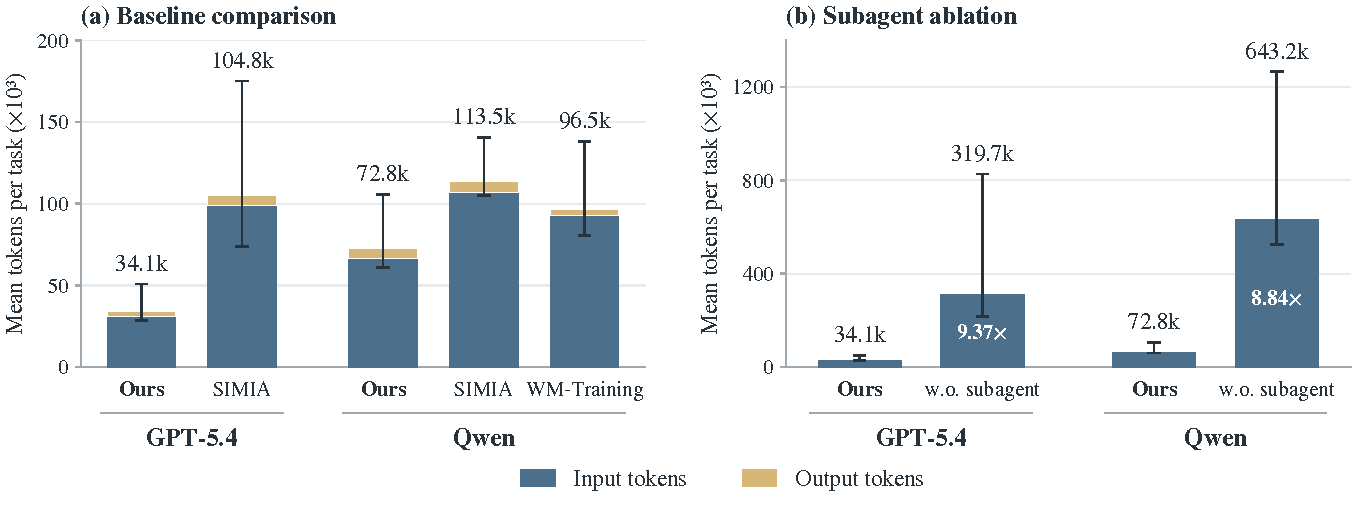
\includegraphics[width=\textwidth]{officebench_token_usage.pdf}
  \caption{\textbf{Estimated token consumption on OfficeBench.}
  Estimated mean cumulative input and output tokens at N=1, including failures.
  GPT-5.4 Ours uses 139 completed tasks, weighted to the benchmark's
  93/300, 95/300, and 112/300 one-, two-, and three-app proportions. This partial
  sample is not random and may underrepresent long unfinished trajectories.
  Qwen B1 uses 12 sampled tasks, with population weighting across
  the same app-count strata; subset sampling uncertainty is separate from the whiskers.
  GPT-5.4 B1, Qwen Ours, and AgentWorld use all 300 tasks.
  Whiskers show low--high modeling scenarios, not confidence intervals.
  (a) GPT-5.4 Ours and B1 use saved AML trajectories with a 40-step limit.
  Qwen-family model variants and step limits differ.
  Ours uses Qwen-AgentWorld-35B-A3B; AgentWorld uses Qwen3.5-35B-A3B.
  (b) Ours without subagent management is the largest counterfactual context
  variant, retaining raw evidence, actor history, and prior world-model transcripts.
  Both bars use each model family's saved Ours trajectories, holding actions,
  modeled calls, and completions fixed; ratios are relative to Ours within
  the same model family.
  Counts use a common tokenizer proxy and modeled missing observations/outputs;
  these are not measured API usage or rerun ablations.}
  \label{fig:officebench-token-usage}
\end{figure*}
